\documentclass{cours}
\usepackage{pgfplots}
\usepackage{multicol}
\usepackage{amssymb}
\usepackage{mathrsfs}
\usetikzlibrary{intersections}
\begin{document}

\setcounter{chapter}{17}

\chapter{Mouvement dans un champ de force centrale conservatif}

\section{Champ de force centrale conservatif}%
\label{sec:champ_de_force_centrale}

\subsection{Définition}%
\label{sub:definition}
\begin{definition}
  Une force centrale est une force portée par une droite qui passe toujours par un même point $O$ fixe. On peut aussi montrer que si la force est conservative, alors sa norme ne dépend que de $r$. En coordonnées polaires, une force centrale conservative s'écrit :
  \begin{equation}
   \vv{F} = F(r) \ver
  \end{equation}
\end{definition}
L'énergie potentielle $E_p$ associée à la force $\vv{F}$ ne dépend elle aussi que de $r$. La variation d'énergie potentiel d'un point matériel $M$ lors d'un déplacement élémentaire $\D \vv{OM} = \D r \ver +r\D \theta \vet$ est
\begin{equation}
  \D E_p = -\vv{F}\cdot\D \vv{OM} = -F(r) \D r
\end{equation}
et on obtient la relation entre énergie potentielle et force :
\begin{eqencadre}
  F(r) = -\frac{\D E_p}{\D r} 
\end{eqencadre}

\subsection{Propriétés du mouvement}%
\label{sub:proprietes_du_mouvement}

Le caractère central de la force appliquée a des conséquences importantes sur le mouvement du point $M$. 

Appliquons le théorème du moment cinétique au point $M$ soumis à une force centrale $\vv{F}$. On a 
\begin{equation}
  \dt{\vv*{L}{O}(M)} = \vv*{\mathcal{M}}{O}(\vv{F}) = \vv{OM}\wedge\vv{F} = r \ver \wedge F(r) \ver = 0
\end{equation}
Et donc on a 
\begin{eqencadre}
  \vv*{L}{O}(M)=\vv{OM}\wedge m\vv{v} = \text{constante}
\end{eqencadre}

La première conséquence importante de la conservation du moment cinétique du point $M$ est que le vecteur $\vv{OM}$ se trouve toujours dans le plan perpendiculaire à $\vv*{L}{O}(M)$, donc \textbf{le mouvement du point $M$ est plan}.

En coordonnées polaires (dans le plan du mouvement), on a $\vv{OM}=r\ver$ et $\vv{v} = \dot{r}\ver + r \dot{\theta}\vet$, donc 
\begin{equation}
  \vv*{L}{O}(M) = \vv{OM} \wedge m\vv{v} = mr^2\dot{\theta}\vez = \text{constante} 
\end{equation}

On en conclut que 
\begin{eqencadre}
  \mathscr{C} = r^2 \dot{\theta}  
\end{eqencadre}
est une constante du mouvement que l'on appelle la \textbf{constante des aires}, voyons pourquoi. Pendant un temps très court $\D t$, le point $M$ se déplace de $\D \vv{OM} =  \D r \ver + r\D \theta \vet$. On représente ce déplacement sur la figure suivante
\begin{center}
  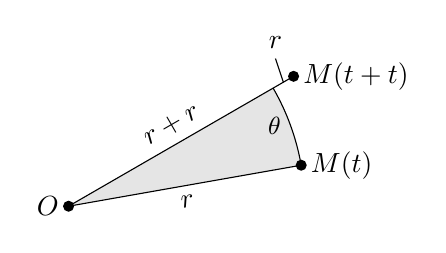
\begin{tikzpicture}
  %tikz meca
    \coordinate (O) at (0,0);
    \coordinate (M) at (10:3);
    \coordinate (Mp) at (30:3.3);
    \fill[gray!20] (O) -- (M) arc(10:30:3);
    \draw (O) node[left]{$O$} --node[below, sloped]{$r$} (M) node[right] {$M(t)$};
    \draw (O) -- node[above, sloped]{$r+\D r$} (Mp) node[right] {$M(t+\D t)$};
    \draw (M) arc(10:30:3) node[midway, left ]{\small $\D \theta$ };
    \fill (M) circle(2pt);
    \fill (Mp) circle(2pt);
    \fill (O) circle(2pt);
    \draw (30:3.15) -- ++(-0.1, 0.3) node[above] {$\D r$}; 
  \end{tikzpicture}
\end{center}

Comme on a $\D r \ll r$, on peut assimiler l'aire balayée par le vecteur $\vv{OM}$ pendant le temps $\D t$ à la portion de disque grisée sur le schéma ci-dessus. Cette aire vaut
\begin{equation}
  \D A = \pi r^2 \frac{\D \theta}{2 \pi} = \frac{1}{2}r^2 \D\theta
\end{equation}
en divisant par $\D t$, on obtient l'aire balayée par unité de temps (en \si{\square\meter\per\second}), ou \textbf{vitesse aréolaire} :
\begin{eqencadre}
  \dt{A} = \frac{1}{2}r^2 \dot{\theta} = \frac{1}{2}\mathscr{C}
\end{eqencadre}
Donc la vitesse aréolaire est constante et vaut $\frac{1}{2}\mathscr{C}$. C'est la \textbf{loi des aires}, ou \textbf{deuxième loi de Kepler} 

\subsection{Étude du mouvement radial, énergie potentielle effective}%
\label{sub:etude_du_mouvement_radial_energie_potentielle_effective}
On étudie un mouvement conservatif, donc l'énergie mécanique du système est conservée :
\begin{equation}
  E_m = E_c + E_p = \text{constante}  
\end{equation}
L'énergie cinétique est $\frac{1}{2}mv^2$, et avec $\dot{r}\ver + r\dot{\theta}\vet$ on obtient
\begin{equation}
  E_m = \frac{1}{2}m \dot{r}^2 + \frac{1}{2}m(r \dot{\theta})^2 + E_p(r)
\end{equation}
On fait apparaître la constante des aires $\mathscr{C} = r^2 \dot{\theta}$ pour obtenir
\begin{equation}
  E_m = \frac{1}{2}m \dot{r}^2 + \underbrace{\frac{1}{2}m\frac{\mathscr{C}^2}{r^2} +E_p(r)}_{E_{p,\text{eff}}(r)} = \frac{1}{2}m \dot{r}^2 + E_{p,\text{eff}}(r)
\end{equation}
En faisant apparaître \textbf{l'énergie potentielle effective} $E_{p,\text{eff}}(r)$, on a fait disparaitre $\theta$ de l'expression de $E_m$ et on se ramène à l'étude du mouvement unidimensionnel d'un point $M$ soumis à une énergie potentielle :
\begin{eqencadre}
  E_{p,\text{eff}}(r)=\frac{1}{2}m\frac{\mathscr{C}^2}{r^2} +E_p(r)
\end{eqencadre}
On pourra appliquer les méthodes énergétiques du chapitre~14 pour étudier le mouvement radial du point $M$.  Et notamment, nous verrons que selon la valeur de l'énergie mécanique la trajectoire de $M$ peut être bornée (état lié) ou non (état de diffusion).



\section{Attraction gravitationnelle}%
\label{sec:champ_newtonien_lois_de_kepler}
Un cas très important de champ de force centrale est celui de l'attraction gravitationnelle entre objets massifs. C'est elle qui gouverne les mouvements des planètes, satellites, galaxies, ...


\subsection{Champ de force newtonien}%
\label{sub:champ_de_force_newtonien}
On considère un point matériel $M$ de masse $m$ soumis à l'attraction gravitationnelle d'un autre point $S$ de masse $m_S$, situé en $O$. La force exercée par $S$ sur $M$ est :
\begin{eqencadre}
  \vv{F} = -G\frac{m\,m_S}{r^2}\ver
\end{eqencadre}
Dans tout ce qui suit, on considérera que $m_S\gg m$. Dans ces conditions on pourra supposer que le point $S$ n'est pas mis en mouvement par la force gravitationnelle exercée par $M$. Le point $S$ restera immobile en $O$.  

L'énergie potentielle associée à la force $\vv{F}$ est :
\begin{eqencadre}
  E_p(r) = -G\frac{m\,m_S}{r}
\end{eqencadre}

\subsection{Mouvement radial}%
\label{sub:mouvement_radial}
Connaissant l'expression de l'énergie potentielle, on peut déterminer celle de l'énergie potentielle effective :
\newcommand{\Epeff}{E_{p,\text{eff}}}
\begin{eqencadre}
  \Epeff(r) = \frac{1}{2}m \frac{\mathscr{C}^2}{r^2}-G\frac{m\,m_S}{r}
\end{eqencadre}
Une étude de la fonction $\Epeff(r)$ montre que : 
\begin{itemize}
  \item $\displaystyle\lim_{r\rightarrow 0} \Epeff(r) = \infty$ ;
  \item $\displaystyle\lim_{r\rightarrow \infty} \Epeff(r) = 0$
  \item $\Epeff(r)$ admet un minimum en $r_0=\frac{\mathscr{C}^2}{Gm_S}$, et $E_\text{min}=-\frac{1}{2}\frac{Gm\,m_S}{r_0}$  
\end{itemize}
On obtient alors l'allure suivante pour $\Epeff(r)$:
\begin{center}
  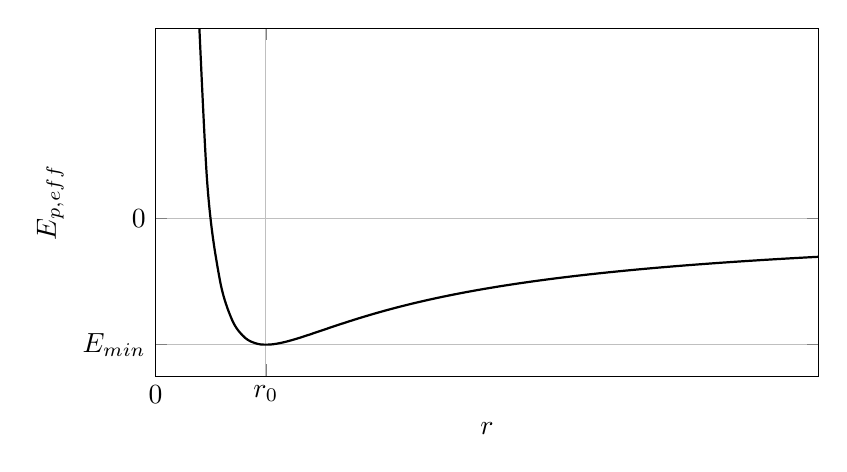
\begin{tikzpicture}
  %tikz meca
    \begin{axis}[
    height=6cm,
    width=10cm,
    xmin=0, xmax=6,
    ymax=1.5,
    grid=major,
    ylabel=$E_{p,\text{eff}}$,
    xlabel=$r$,
    xtick = {0,1},
    xticklabels={$0$, $r_0$},
    ytick = {-1, 0},
    yticklabels={ $E_\text{min}$,$0$},
    ]
    \addplot[domain=0.35:6, samples=50, smooth, thick] {(1/x^2-2/x)};      
    \end{axis}
  \end{tikzpicture}
  \captionof{figure}{Diagramme énergétique radiale pour un corps soumis à un champ de force newtonien\label{fig:diag_energie}}
\end{center}

On a alors différents mouvements possibles en fonction de l'énergie mécanique du système :
\begin{itemize}
  \item Si $E_m = E_\text{min}$, le système se trouve au minimum d'énergie potentielle, donc $r$ est constant, le mouvement est circulaire. Comme le moment cinétique est constant, le mouvement est circulaire uniforme ;
  \item Si $E_\text{min}<E_m<0$, la trajectoire est bornée, le point $M$ reste à proximité de $S$, Le système est dans un état lié, dans ce cas on admettra que le mouvement de $M$ est une ellipse dont $S$ est l'un des foyers. C'est la \textbf{première loi de Kepler}. 
  
  L'équation cartésienne d'une ellipse est :
  \begin{equation}
    \left(\frac{x}{a}\right)^2 + \left( \frac{y}{b} \right)^2 = 1  
  \end{equation}
  $a$ et $b$ sont respectivement le demi grand axes et le demi petit axe de l'ellipse. L'équation polaire de l'ellipse donc le grand axe est aligné avec la direction $\theta=0$ est:
  \begin{equation}
    r(\theta) = \frac{p}{1+e\cos(\theta)}
  \end{equation}
  $p$ est le paramètre de l'ellipse et $e$ est son excentricité.
  \item Si $E_m\geq0$, la trajectoire n'est plus bornée, le point $M$ peut s'éloigner arbitrairement loin de $S$, c'est un état de diffusion. La trajectoire est une parabole ($E_m=0$) ou une hyperbole ($E_m>0$).  
\end{itemize}

\subsection{Énergie mécanique}%
\label{sub:energie_mecanique}
Considérons une trajectoire bornée, c'est à dire que $E_\text{min}<E_m<0$. On sait que dans ce cas, l'orbite est elliptique et les valeurs extrêmes de $r$ sont notées $r_1$ et $r_2$. 

\begin{minipage}{\linewidth}
\begin{center}
  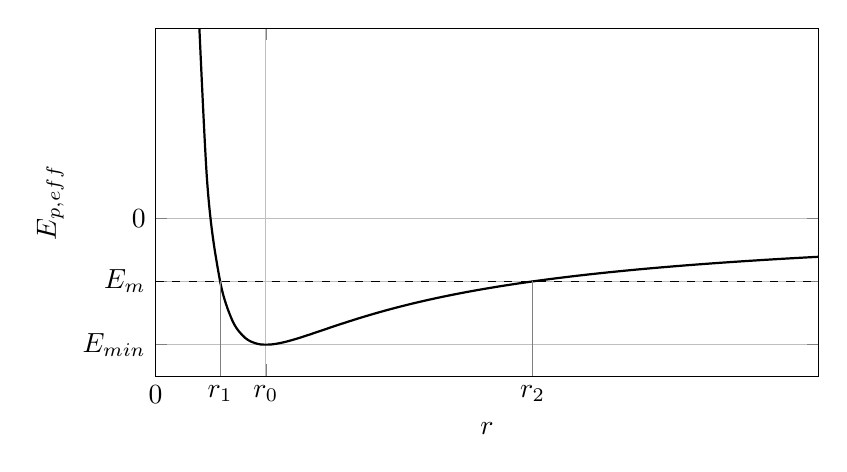
\begin{tikzpicture}
  %tikz meca
    \begin{axis}[
    height=6cm,
    width=10cm,
    xmin=0, xmax=6,
    ymax=1.5,
    grid=major,
    ylabel=$E_{p,\text{eff}}$,
    xlabel=$r$,
    xtick = {0,1},
    xticklabels={$0$, $r_0$},
    ytick = {-1,-0.5, 0},
    yticklabels={ $E_\text{min}$,$E_m$, $0$},
    clip mode=individual,
    ]
    \coordinate (B) at (axis description cs:0,0);
    \addplot[domain=0.35:6, samples=50, smooth, thick, name path=Ep] {(1/x^2-2/x)};
    \draw[dashed, name path=Em] (axis cs:0, -0.5) -- (axis cs:6, -0.5);
    \draw[name intersections={of=Ep and Em},gray] (intersection-1) -- (intersection-1|-B) node[below, color=black]{$r_1$}
    (intersection-2) -- (intersection-2|-B) node[below, color=black]{$r_2$};
    \end{axis}
  \end{tikzpicture}
  \captionof{figure}{Diagramme énergétique radial pour une trajectoire bornée}
\end{center}
\end{minipage}

\begin{center}
  \begin{tikzpicture}
  %tikz meca
   \coordinate (S) at ({-sqrt(5)}, 0);
   \draw[name path=orb] (0,0) circle(3cm and 2cm);
   \fill (S) circle(2pt) node[below, yshift=-2pt]{$S$};
   \draw[latex-latex] (-3, 0) -- node[below]{$2a$} (3,0); 
   \path[name path=l] (0,0) -- (2,2);
   \fill[name intersections={of=orb and l}] (intersection-1) coordinate(M) circle(2pt) node[above right] {$M$};
   \draw ($(S)!0.5!(-3,0)$) node[above]{$r_1$};
   \draw ($(S)!0.5!(3,0)$) node[above]{$r_2$};
  \end{tikzpicture}
  \captionof{figure}{Trajectoire elliptique, grand axe $2a$ et valeurs extrêmes de $r$. On a $2a = r_1+r_2$.}
\end{center}

On trouve $r_1$ et $r_2$ en écrivant 
\begin{equation}
  E_m = \Epeff(r_{1,2})
\end{equation}
Donc $r_1$ et $r_2$ sont solutions de l'équation 
\begin{equation}
  \Epeff(r) = \frac{1}{2}m \frac{\mathscr{C}^2}{r^2}-G\frac{m\,m_S}{r} = E_m \Leftrightarrow 2E_mr^2 + 2Gm\, m_Sr -m\mathscr{C}^2 = 0
\end{equation}
Les deux solutions de cette équation satisfont 
\begin{equation}
  r_1 + r_2 = 2a = -\frac{2Gm\,m_S}{2E_m}= -\frac{Gm\,m_S}{E_m}
\end{equation}
dont on déduit l'expression de l'énergie mécanique en fonction du demi grand axe $a$ de l'ellipse :
\begin{eqencadre}
  E_m = -\frac{G m\,m_S}{2a} 
\end{eqencadre}
Si le mouvement est circulaire, on a $a=r$ et 
\begin{equation}
  E_m = -\frac{Gm\, m_S}{2r}
\end{equation}



\subsection{Étude du mouvement circulaire}%
\label{sub:etude_du_mouvement_circulaire}
On a vu dans la partie précédente que si l'énergie potentielle effective du point $M$ est minimale, alors la trajectoire de $M$ est circulaire uniforme autour de $S$. L'accélération du point $M$ en coordonnées polaires est :
\begin{equation}
  \vv{a} = -\frac{v^2}{r}\ver
\end{equation}
Le principe fondamental de la dynamique appliqué au point $M$, donne alors :
\begin{equation}
  -m\frac{v^2}{r} = -G\frac{m\, m_S}{r^2}  
\end{equation}
Donc la vitesse du point $M$ lorsqu'il suit une trajectoire circulaire de rayon $r$ autour de $S$ est
\begin{eqencadre}
  v = \sqrt{\frac{Gm_S}{r}}
  \label{eq:vitesse_orbite}
\end{eqencadre}

On peut en déduire la période de rotation de $M$ autour de $S$ :
\begin{equation}
  T = \frac{2\pi r}{v} = \frac{2\pi}{\sqrt{Gm_S}}r^\frac{3}{2}
\end{equation}

On en déduit la \textbf{troisième loi de Kepler} :
\begin{eqencadre}
  \frac{T^2}{r^3} = \frac{4\pi^2}{Gm_S}
\end{eqencadre}

Il est intéressant de noter que cette valeur ne dépend que de la masse de $S$ et non de celle de $M$. Donc la valeur de $\frac{T^2}{r^3}$ sera la même pour tous corps ayant une orbite circulaire autour de $S$.

On peut généraliser cette formule à toutes les orbites elliptiques en replaçant le rayon $r$ par le demi grand axe $a$ de l'ellipse :
\begin{eqencadre}
  \frac{T^2}{a^3} = \frac{4\pi^2}{Gm_S}
\end{eqencadre}


\subsection{Satellite géostationnaire}%
\label{sub:satellite_geostationnaire}
Un satellite geostationnaire est un satellite artificiel de la Terre qui reste à la verticale d'un point fixe à la surface de la Terre. Il est très utile d'avoir un satellite geostationnaire car il occupe une position apparente fixe ce qui rend les communications plus faciles car on peut pointer une antenne parabolique fixe dans sa direction.

Pour qu'il soit géostationnaire, il faut que l'orbite du satellite soit dans le plan de l'équateur, car il doit tourner autour du même axe que la Terre. 

Comme la Terre tourne sur elle-même à vitesse constante, il faut que le satellite parcourt son orbite également à vitesse constante, L'orbite doit donc être circulaire.

Enfin, il faut que la vitesse angulaire de rotation du satellite autour de la Terre soit égale à la vitesse angulaire de rotation de la Terre sur elle-même. 

Attention, la période de rotation de la Terre sur elle-même n'est pas de \SI{24}{\hour} ! La Terre met \SI{24}{\hour} à retrouver la même orientation par rapport au Soleil, mais comme elle tourne autour du Soleil dans le même sens que son sens de rotation, ce temps est légèrement plus grand que sa période de rotation.
\begin{center}
  \begin{tikzpicture}
  %tikz meca
  \def\r{2cm}
  \def\rt{0.4}
    \coordinate (S) at (0,0);
    \draw (S) circle(\r);
    \draw[fill=white] ($(S)+(30:\r)$) coordinate (T1) circle(\rt);
    \draw[fill=white] ($(S)+(60:\r)$) coordinate (T2) circle(\rt);
    \foreach \a in {0,30,...,330}{
      \draw[gray] (T1) -- ++(\a:\rt);
      \draw[gray] (T2) -- ++(\a:\rt);
    }
    \draw[fill=black] ($(T1)+(-150:\rt)$) coordinate (P1) circle(1pt); 
    \draw[fill=black] ($(T2)+(-120:\rt)$) coordinate (P2) circle(1pt); 
    \draw[gray] 
    (S) -- (P1)
    (S) -- (P2);
    \fill (S) circle(2pt) node[below, yshift=-2pt]{Soleil};
    \draw (S) ++(30:0.5) arc(30:60:0.5) node[midway, above right]{$\alpha$};

    \draw[gray] (T2) -- ++(-150:0.6);
    \draw (T2) ++(-150:0.5) arc(-150:-120:0.5) node[midway, below left]{$\alpha$};
  \end{tikzpicture}
  \captionof{figure}{Deux positions de la Terre par rapport au Soleil séparées par un jour solaire. On remarque qu'elle a tourné d'un angle $\alpha$ supplémentaire par rapport à son orientation initiale.\label{fig:jour_sideral}}
\end{center}

La période $T_0$ de rotation de la Terre (jour sidéral) est égale à la durée $T_S$ d'un jour solaire moins le temps pris pour tourner de l'angle $\alpha$ représenté sur la figure~\ref{fig:jour_sideral}. Si $T_R$ est la période de révolution de la Terre autour du Soleil, la vitesse angulaire de rotation de la Terre est :
\begin{equation}
  \omega_0 = \frac{2\pi}{T_0} = \frac{2\pi + \alpha}{T_S} \quad \text{soit} \quad T_0 = \frac{1}{1+\alpha/2\pi}T_S
\end{equation}
$\alpha$ correspond à $1/365$ tour, soit $\alpha=\frac{2\pi}{365}$ et on a finalement :
\luaexec{T0 = 1/(1+1/365)*24*3600}
\begin{equation}
  T_0 = \frac{1}{1+1/365}T_S \approx \luaexec{SI(T0, 0, "\\second")}
\end{equation}
En utilisant la troisième loi de Kepler, on trouve que le rayon de l'orbite géostationnaire est 
\luaexec{rgeo = (_G*_m_T*T0^2/4/_pi^2)^(1/3)}
\begin{equation}
  r_\text{geo}=\left( \frac{G m_T T_0^2}{4\pi^2} \right)^{\frac{1}{3}} \approx \luaexec{SI(rgeo/1000, 0, "\\kilo\\meter")} 
\end{equation}
où $m_T$ est la masse de la Terre. Si on retranche le rayon $r_T$  de la Terre pour connaitre l'altitude du satellite, on obtient 
\begin{equation}
  h_\text{geo} = r_\text{geo}-r_T \approx \luaexec{SI((rgeo-_r_T)/1000, 0, "\\kilo\\meter")}
\end{equation}
%
On retiendra que l'altitude d'un satellite geostationnaire est d'environ \SI{36000}{\kilo\meter}.

\subsection{Vitesses cosmiques}%
\label{sub:vitesses_cosmiques}
Les vitesses cosmiques sont des vitesses particulières pour un corps soumis à l'attraction gravitationelle d'un autre corps. 

La première est la vitesse minimale $v_1$ pour mettre en orbite un satellite autour de la Terre. Dans ce cas, le rayon de l'orbite est le rayon de la Terre $r_T$ et l'équation~\eqref{eq:vitesse_orbite} donne la vitesse nécessaire pour avoir une orbite circulaire (une orbite elliptique a une énergie mécanique supérieure et demanderait donc une vitesse plus grande). On obtient :
\begin{equation}
  v=\sqrt{\frac{Gm_T}{r_T}}\approx \luaexec{SI((_G*_m_T/_r_T)^0.5, 0, "\\meter\\per\\second")}\approx \luaexec{SI((_G*_m_T/_r_T)^0.5/1000, 0, "\\kilo\\meter\\per\\second")}
\end{equation}
 
 La seconde vitesse cosmique est la vitesse de libération $v_l$ , c'est la vitesse minimale à donner pour que le corps puisse s'éloigner arbitrairement loin de la Terre. Il faut donc lui donner suffisamment d'énergie pour qu'il puisse s'éloigner à l'infini de la Terre en partant de sa surface. On peut utiliser la conservation de l'énergie mécanique entre un point $A$ à la surface de la Terre et un point $B$ situé à l'infini :
 \begin{equation}
   E_m(A) = E_p(A) + E_c(A) = -\frac{Gm\, m_T}{r_T} + \frac{1}{2}mv_l^2= E_m(B) = E_p(B) + E_c(B) = 0
 \end{equation}

 On obtient alors 
 \begin{equation}
   v_l=\sqrt{\frac{2Gm_T}{r_T}}=\sqrt{2}v_1\approx\luaexec{SI((2*_G*_m_T/_r_T)^0.5, 0, "\\meter\\per\\second")}\approx \luaexec{SI((2*_G*_m_T/_r_T)^0.5/1000, 0, "\\kilo\\meter\\per\\second")}
 \end{equation}


 \section{Détermination numérique de la trajectoire}%
 \label{sec:determination_numerique_de_la_trajectoire}
 
 On peut déterminer la trajectoire d'un point matériel dans un champ de force newtonien analytiquement (voir partie~\ref{sec:demo_ellipse}). Mais dans le cas général, c'est plus compliqué. On peut cependant calculer numériquement la trajectoire dans un champ de force conservatif. Il suffit de résoudre numériquement l'équation différentielle du mouvement obtenue à partir du PFD.

 La principe fondamental de la dynamique conduit à l'équation 
 \begin{equation}
   \vv{a} = \frac{F(r)}{m} \ver = \frac{F(r)}{m} \frac{\vv{r}}{||\vv{r}||}
 \end{equation}

 On utilse le code suivant :

 \begin{minted}{python}
import numpy as np
from scipy.integrate import solve_ivp
import matplotlib.pyplot as plt
from matplotlib.animation import FuncAnimation # Pour faire une animation

# Définition de l'équation différentielle à résoudre 
# Y est une liste de 6 valeurs [x, y, z, dx/dt, dy/dt, dz/dt]
# la fonction renvoie la liste dY/dt
def F(t, Y):
    K = 0.1
    res = np.array(Y)
    for i in range(3):
        res[i] = Y[i+3]
    pos = np.array(Y[0:3])
    r = np.sqrt(np.sum([pos[i]**2 for i in range(3)]))
    for i in range(3):
        res[3+i] = -K/r**2*pos[i]/r
    return res

fig, ax = plt.subplots()

# Conditions initiales [x0, y0, z0, vx0, vy0, vz0]
Y0 = np.array([-1, 0, 0, 0.2, 0.2, 0])
tlims = [0, 80]
teval = np.linspace(0, 80, 2000)
# Résolution numérique de l'équation différentielle
sol = solve_ivp(F, tlims, Y0, t_eval=teval, method='Radau')

pl, = plt.plot([], [])
xdata = []
ydata = []

# Symbolise le centre de force
cercle = plt.Circle((0,0), 0.06, color='r')
ax.add_patch(cercle)

# Le point matériel soumis à la force
planete = plt.Circle((1,0), 0.03, color='b')
ax.add_patch(planete)

# Les deux fonctions suivantes servent à animer le mouvement du point matériel
# ça n'est pas strictement nécessaire, mais c'est joli
def init():
    ax.set_xlim(-2,2)
    ax.set_ylim(-2,2)
    return pl, planete

def update(frame):
    xdata.append(sol.y[0,frame])
    ydata.append(sol.y[1,frame])
    pl.set_data(xdata, ydata)
    planete.set_center((xdata[-1], ydata[-1]))
    return pl,planete,

ani = FuncAnimation(fig, update, frames=range(len(sol.t)),
                    init_func=init, blit=True, interval=20)
plt.show()
 \end{minted}
On peut alors simuler la trajectoire d'un point matériel soumis à un champ de force de la forme
\begin{equation}
  F(r) = \frac{K}{r^\alpha}
\end{equation}
Avec des conditions initiales bien choisies, on obtient les résultats suivants
\begin{center}
\begin{tikzpicture}
  \begin{axis}[
      width=5cm,
      xshift=-4cm,
      xmin=-2,xmax=1.5,
      ymin=-1.5, ymax=2,
      xtick=\empty,
      ytick=\empty,
      ]
    \addplot[] table {data/force_centrale_1.9.dat};
    \draw[fill] (axis cs:0,0) circle (3pt);
    \draw (axis description cs:1,1) node[below left]{$\alpha=1.9$}; 
  \end{axis}
  \begin{axis}[
      width=5cm,
      xmin=-2,xmax=1.5,
      ymin=-1.5, ymax=2,
      xtick=\empty,
      ytick=\empty,
    ]
    \addplot[] table {data/force_centrale_2.dat};
    \draw[fill] (axis cs:0,0) circle (3pt);
    \draw (axis description cs:1,1) node[below left]{$\alpha=2$}; 
  \end{axis}
  \begin{axis}[
      width=5cm,
      xshift=4cm,
      xmin=-2,xmax=1.5,
      ymin=-1.5, ymax=2,
      xtick=\empty,
      ytick=\empty,
      ]
    \addplot[] table {data/force_centrale_2.1.dat};
    \draw[fill] (axis cs:0,0) circle (3pt);
    \draw (axis description cs:1,1) node[below left]{$\alpha=2.1$}; 
  \end{axis}
  \begin{axis}[
      width=5cm,
      xshift=8cm,
      xmin=-2,xmax=1.5,
      ymin=-1.5, ymax=2,
      xtick=\empty,
      ytick=\empty,
      ]
    \addplot[] table {data/force_centrale_2.5.dat};
    \draw[fill] (axis cs:0,0) circle (3pt);
    \draw (axis description cs:1,1) node[below left]{$\alpha=2.5$}; 
  \end{axis}
\end{tikzpicture}
\end{center}

On remarque que la valeur $\alpha=2$ est particulière, pour cette valeur la trajectoire du point matériel est fermée.
 \section{Démonstration de l'équation de la trajectoire (hors programme)}%
 \label{sec:demo_ellipse}
 
 On considère un champ de force newtonien :
 \begin{equation}
 \vv{F} = -\frac{K}{r^2}\ver \quad E_p = -\frac{K}{r}
 \end{equation}
 La conservation du moment cinétique implique que 
 \newcommand{\cc}{\mathscr{C}}
 \begin{equation}
   \mathscr{C} = r^2 \dot{\theta}
 \end{equation}
 est une constante du mouvement. (voir~\ref{sub:proprietes_du_mouvement}), tout comme l'énergie mécanique
 \begin{equation}
   E_m = \frac{1}{2}mv^2 - \frac{K}{r}
 \end{equation}
 Nous allons réécrire l'énergie mécanique en fonction de $u=\frac{1}{r}$. Pour cela on cherche à exprimer $v^2$ en fonction de $u$.
 On part de l'expression de $\vv{v}$ en coordonnées polaires :
 \begin{equation}
   \vv{v} = \dot{r}\ver + r \dot{\theta}\vet  = \dot{r}\ver + \frac{\cc}{r}\vet = \dot{r}\ver  + \cc u \vet  
 \end{equation} 
Par ailleurs on a
\begin{equation}
  \dot{r}=\dt{r}=\frac{\D r}{\D \theta} \dt{\theta} = \dot{\theta}\frac{\D r}{\D\theta} = \frac{\cc}{r^2}\frac{\D r}{\D\theta} = \cc u^2 \frac{\D r}{\D\theta}
\end{equation}
et
\begin{equation}
  \frac{\D r}{\D\theta} = \frac{\D(\frac{1}{u})}{\D \theta} = -\frac{1}{u^2}\frac{\D u}{\D \theta}
\end{equation}
Donc finalement
\begin{equation}
  \dot{r} = -\cc \frac{\D u}{\D \theta}
\end{equation}
et on obtient
\begin{equation}
  v^2 = \cc^2 \left( \left( \frac{\D u }{\D \theta} \right)^2 + u^2 \right) 
\end{equation}
Donc l'énergie mécanique devient
\begin{equation}
  E_m = \frac{1}{2}\cc^2 m \left( \left( \frac{\D u}{\D \theta} \right)^2 + u^2 \right) - Ku
\end{equation}
Comme l'énergie mécanique est une constante du mouvement, sa dérivée par rapport à $\theta$ est nulle et
\begin{equation}
  \frac{\D E_m}{\D \theta} = 0 = \cc^2 m \left( \frac{\D u}{\D \theta}\frac{\D^2 u}{\D \theta^2} + u \frac{\D u }{\D \theta} \right) -K 
\end{equation}
Comme $\frac{\D u}{\D\theta}$ n'est pas identiquement nul, on obtient l'équation :
\begin{equation}
  \frac{\D^2u}{\D\theta^2} + u = \frac{K}{\cc^2m}
\end{equation}
C'est l'équation différentielle d'un oscillateur harmonique avec un second membre constant. La solution générale est :
\begin{equation}
  u(\theta) = A\cos(\theta-\theta_0) + \frac{K}{m\cc^2} 
\end{equation}
où $A$ et $\theta_0$ sont déterminées par les conditions initiales. On a finalement
\begin{eqencadre}
  r(\theta) = \frac{p}{1+e\cos(\theta-\theta_0)}
\end{eqencadre}
avec $p=\frac{m\cc^2}{K}$ et $e=\frac{Am\cc^2}{K}$. C'est l'équation polaire générale d'une conique. Lorsque $0<e<1$ on a une ellipse. Lorsque $e=1$ c'est une parabole et lorsque $e>1$ c'est une branche d'hyperbole.
\end{document}

